\section{Validación}
 Las motivaciones del empleador han sido comprendidas y se han tomado las consideraciones requeridas para responder a su motivación, para esto se han aplicado funciones como iniciar secion con alguna cuenta, poder visualizar inamegenes en 360° de lugares turisticos, caracteristicos o iconicos de la regien del maule, presentar un diseño que sea relajante, entre otras funciones mencionadas con anterioridad en este documento.
\subsection{Prototipo de validación funcional}
A continuación se presentan algunas capturas de pantalla obtenidas de la aplicación para mostrar el progreso y el diseño realizado por los desarrolladores.
\begin{figure}[H]
	\centering
	\subfloat[Screenshot de la app N°01]
	{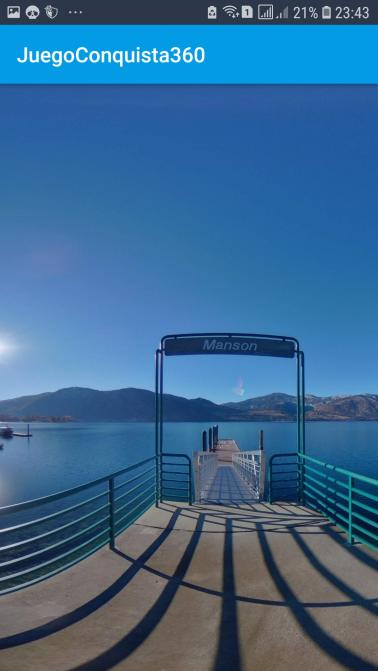
\includegraphics[width=5cm, height=8cm]{imgs/Screenshot1.jpg}}
	\subfloat[Screenshot de la app N°02]
	{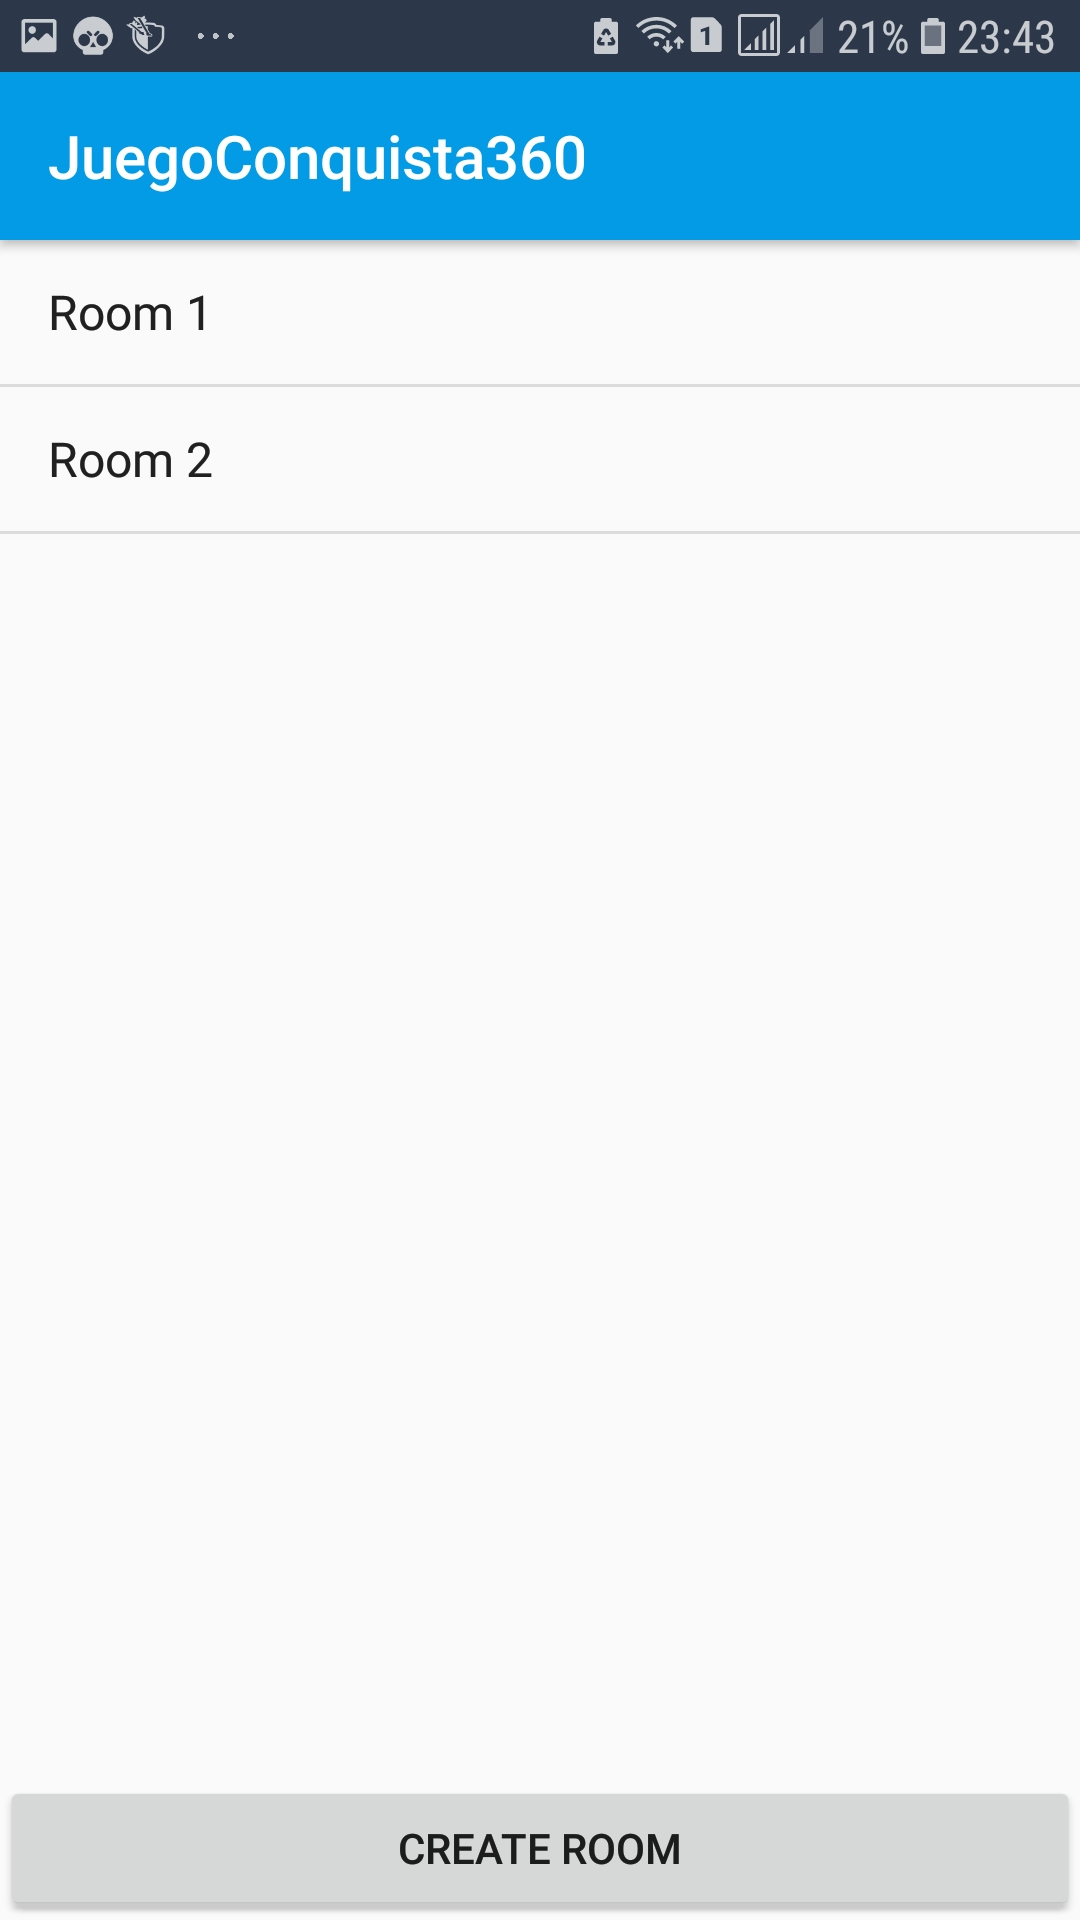
\includegraphics[width=5cm, height=8cm]{imgs/Screenshot2.jpg}}
	\subfloat[Screenshot de la app N°03]
	{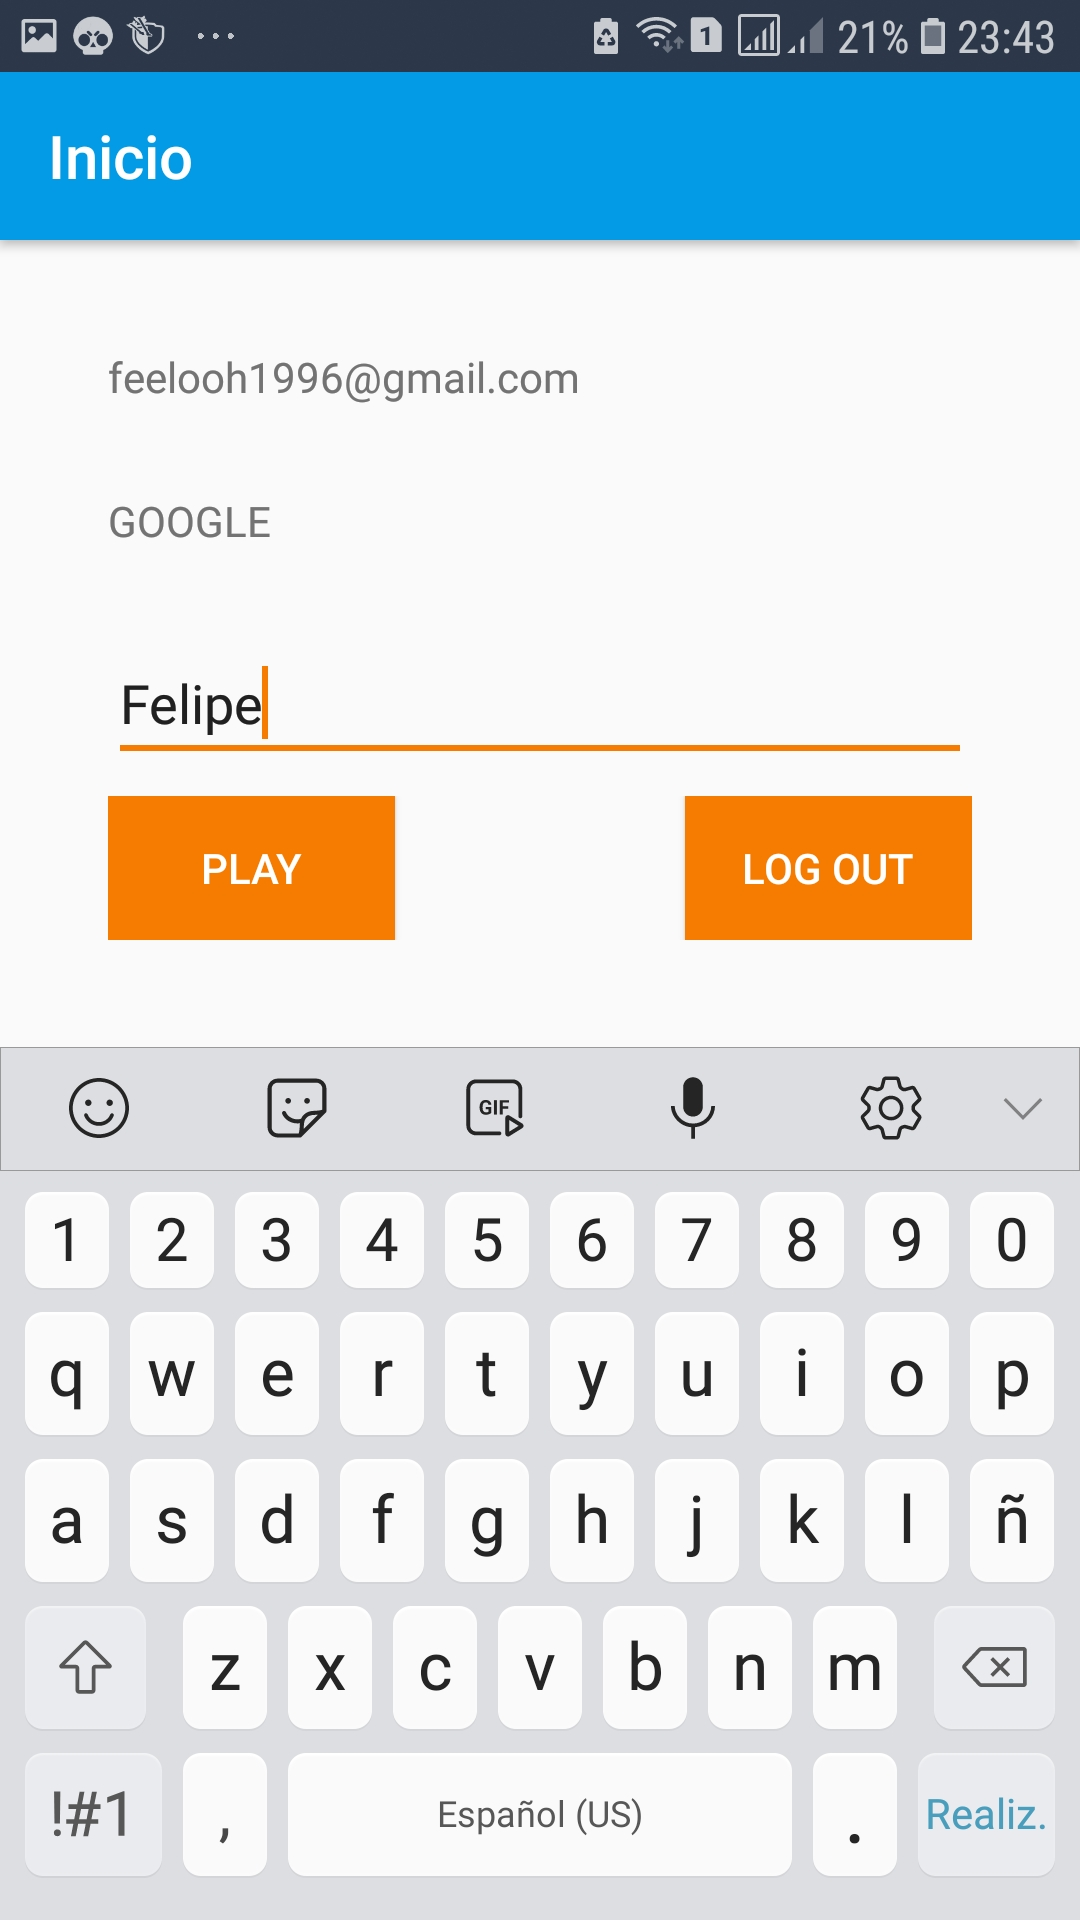
\includegraphics[width=5cm, height=8cm]{imgs/Screenshot3.jpg}}
 	\caption{Screenshot 1, 2 y 3}
\end{figure}
\begin{figure}[H]
	\centering
	\subfloat[Screenshot de la app N°04]
	{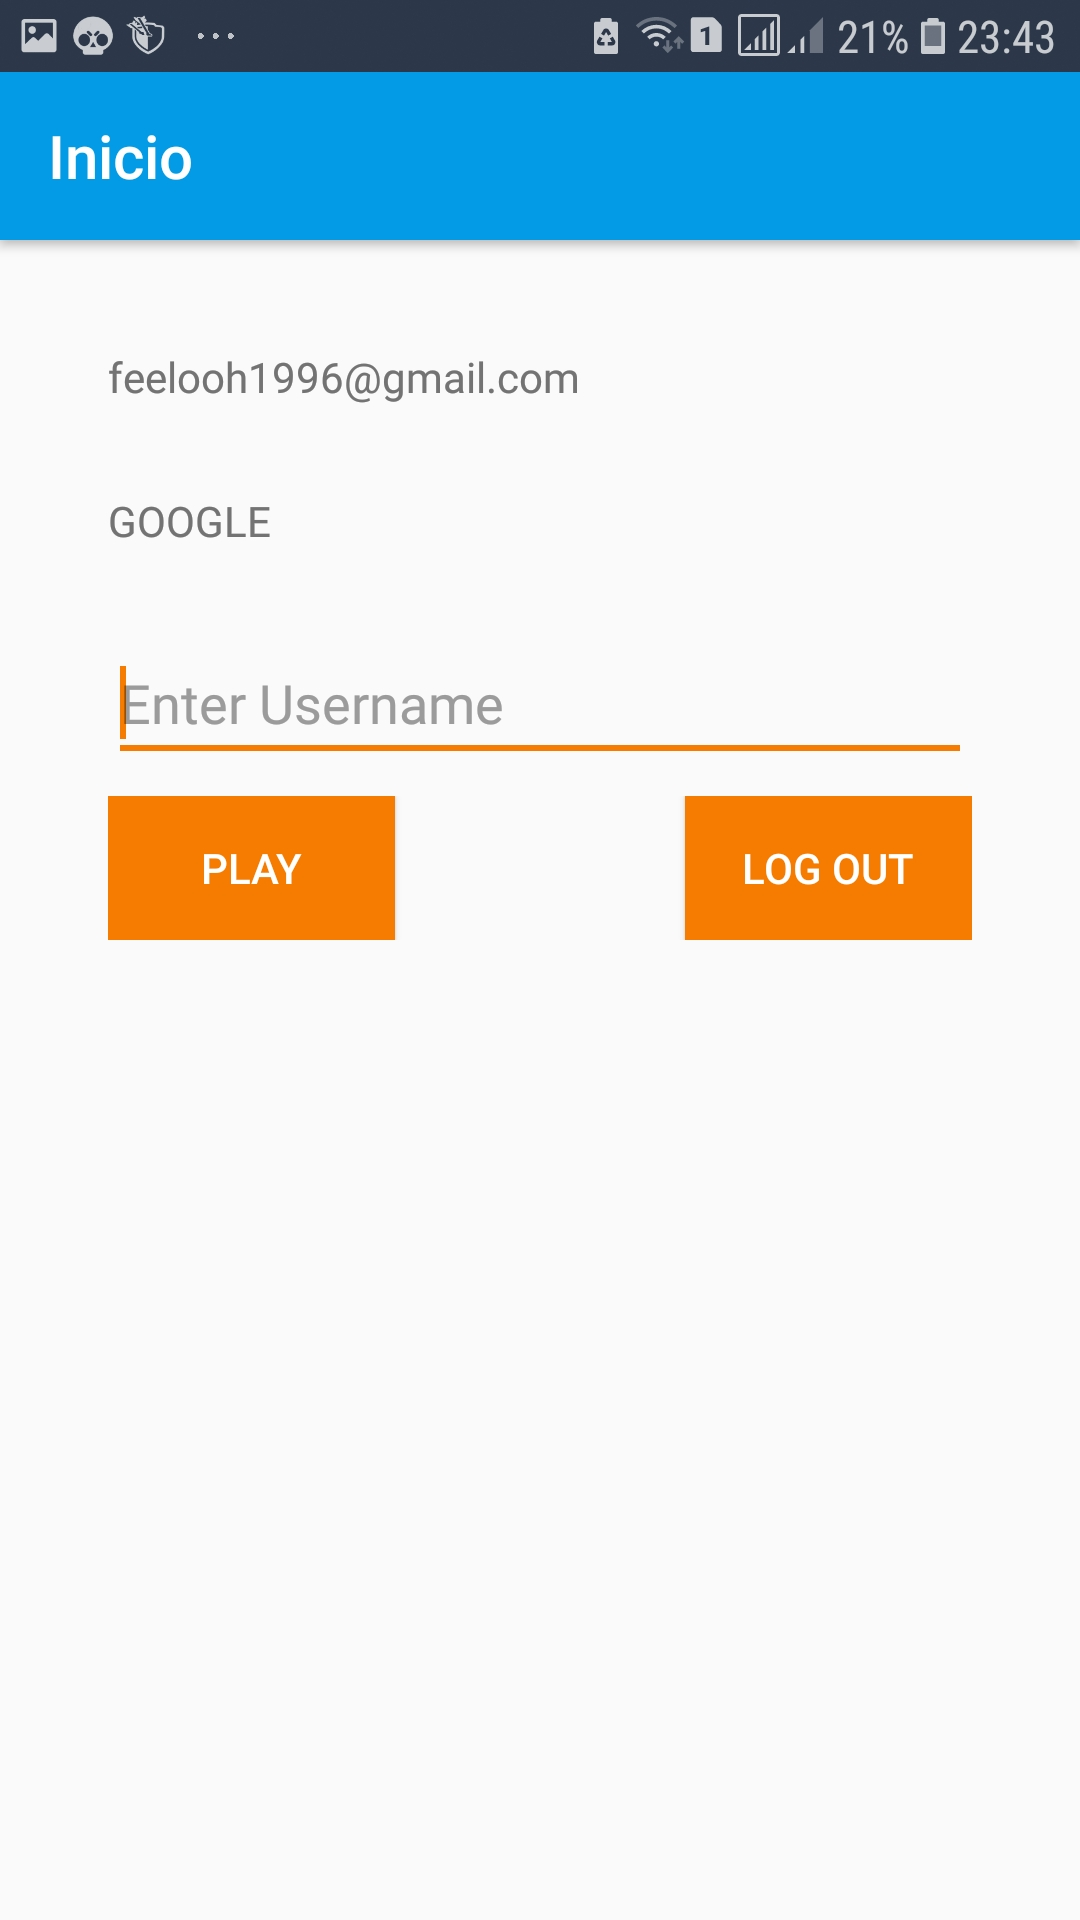
\includegraphics[width=5cm, height=8cm]{imgs/Screenshot4.jpg}}
	\subfloat[Screenshot de la app N°5]
	{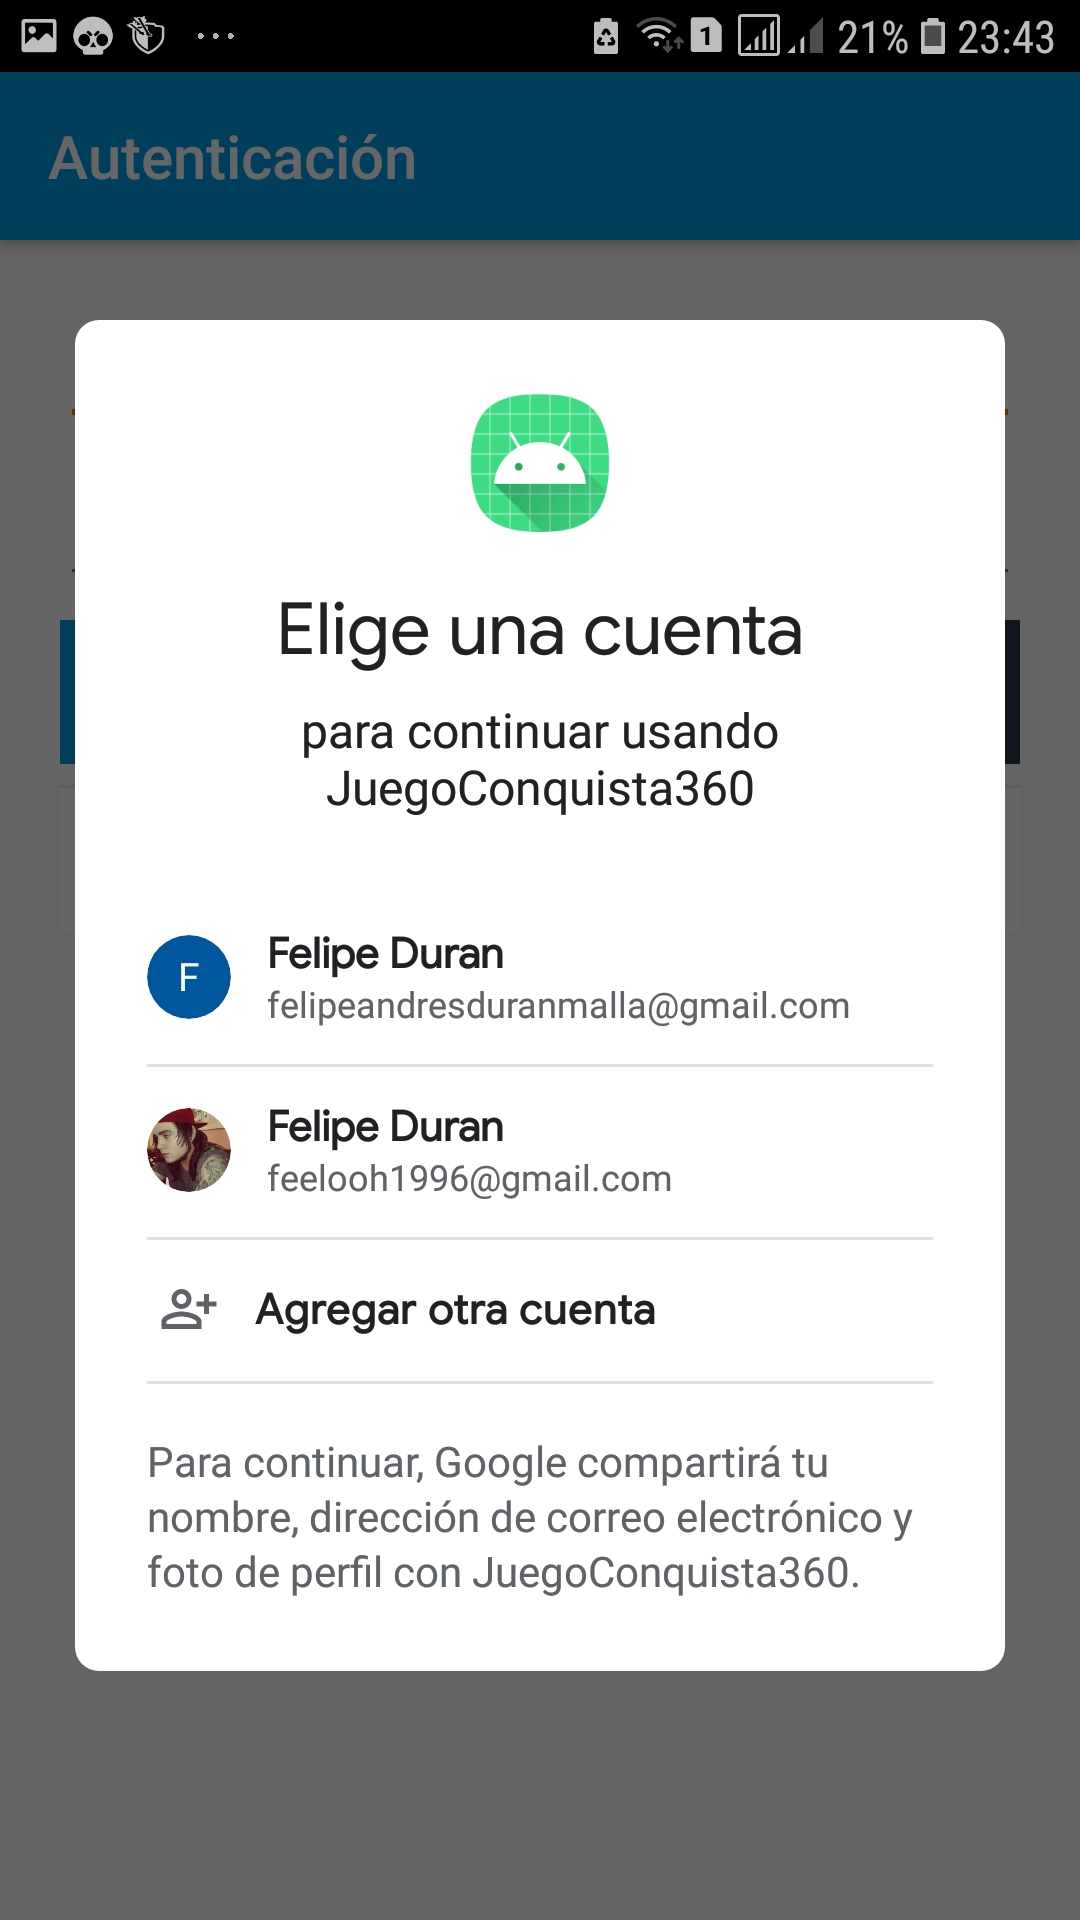
\includegraphics[width=5cm, height=8cm]{imgs/Screenshot5.jpg}}
	\subfloat[Screenshot de la app N°6]
	{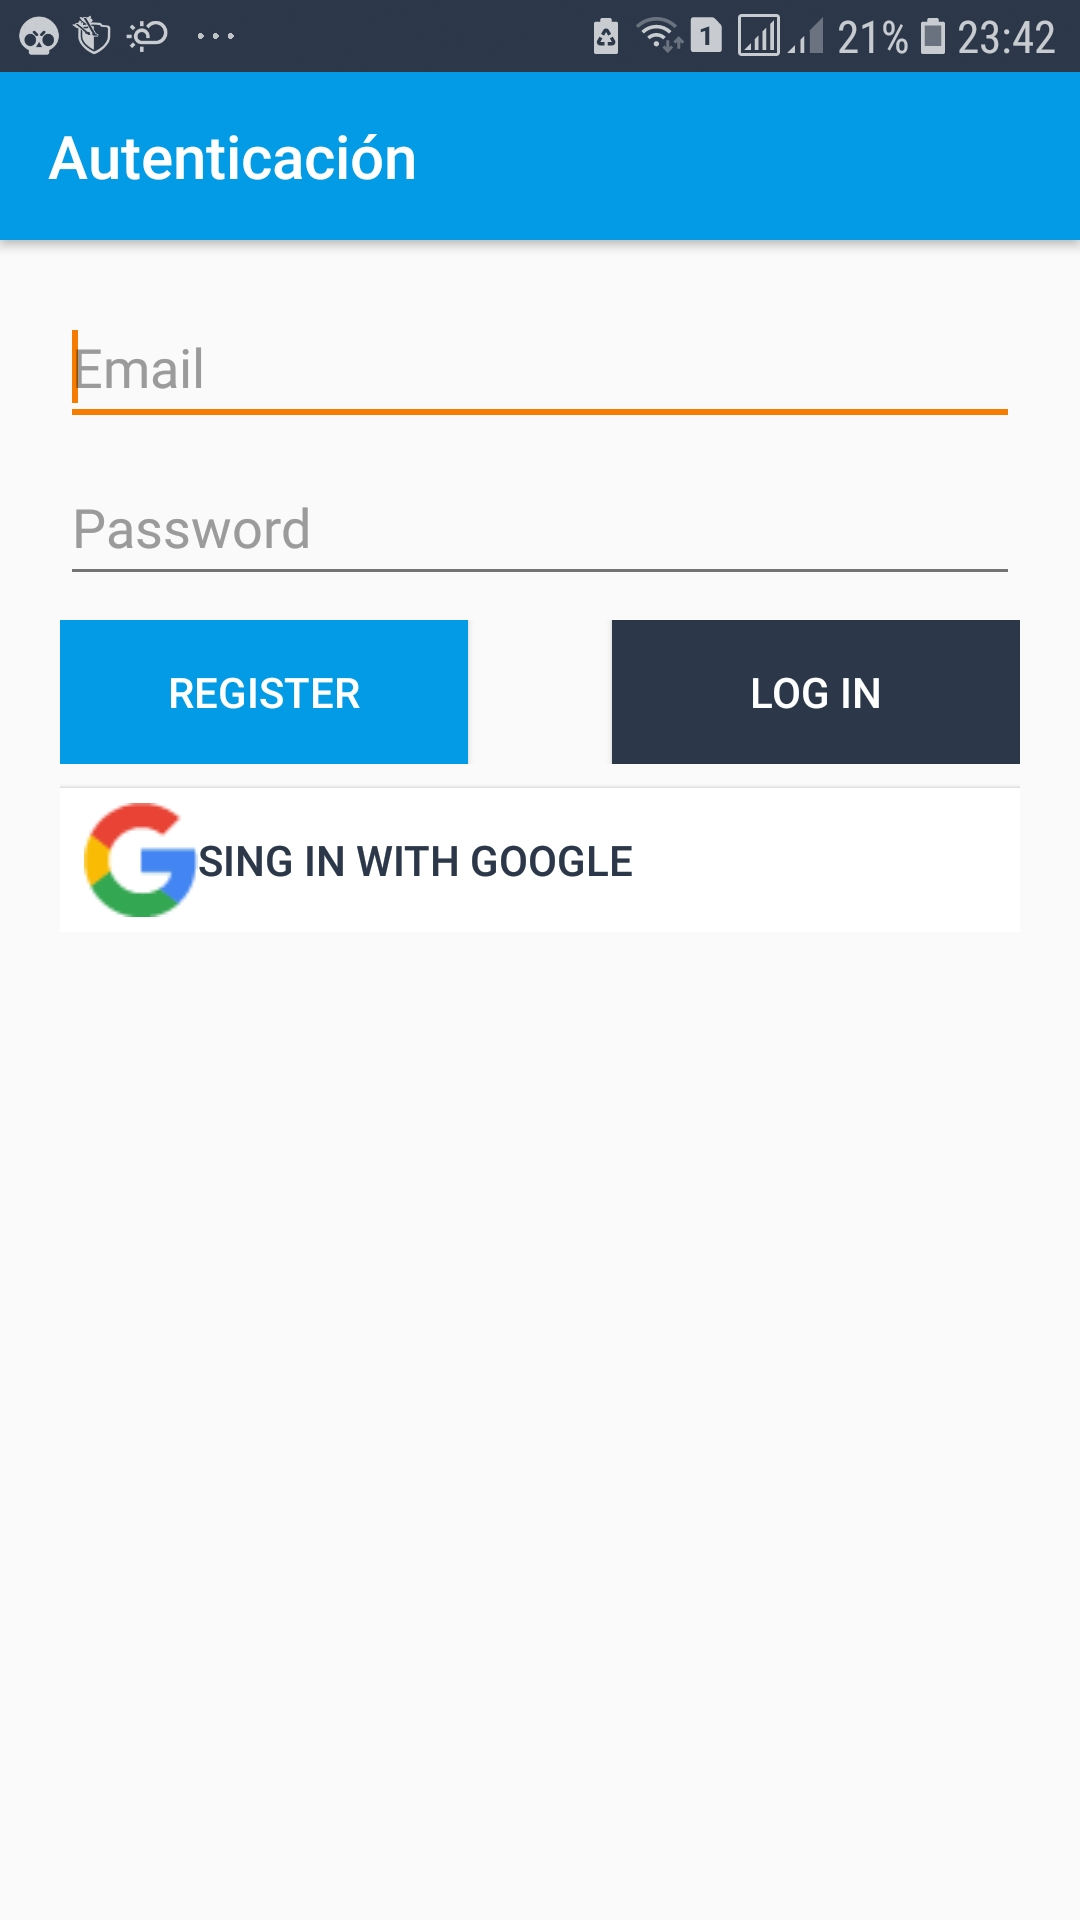
\includegraphics[width=5cm, height=8cm]{imgs/Screenshot6.jpg}}
 	\caption{Screenshot 4, 5 y 6}
\end{figure}

